In den ersten Versuchen geht es darum ein Verständnis für das Druck-Geschwindigkeit-Gesetz und für die verwendeten Messmetoden zu bekommen.

\section{Beobachtungen mit Sonden}

Im ersten Versuchsteil geht es darum geeignete Messmethoden und entsprechende Sonden für die Messung für statischen, dynamischen und Gesamtdruck zu finden. Dafür werden jeweils die beiden zu prüfenden Sonden (Rohr- und Scheibensonde) parallel und senkrecht zum Luftstrom ausgerichtet und dann, am angeschlossenen Manometer, der entsprechende Druck abgelesen. Die ermittelten Werte sind in Tabelle \ref{tab:TabelleD1} zu finden. Aus diesen lässt sich erkenne, dass die Werte für die parallelen Messungen nahezu gleich sind, wobei sich die Messwerte für die Senkrechte Messung stark unterscheiden, dies lässt sich mit den Verwirbelungen an der Kante der Öffnung der Rohrsonde erklären. Da die Kante bei der Scheibensonde weiter von der Öffnung entfernt ist, ist am Ort der Öffnung eine weniger starke Verwirbelung, was sich positiv auf den Messwert auswirkt. Dadurch, dass die Öffnung bei der parallelen Messung zur Strömung hin gedreht ist, wird hierbei auch der dynamische Druck gemessen, demnach wird also hierbei der Gesamtdruck gemessen. Bei der senkrechten Orientierung wird also die dynamische Komponente ausgespart und man misst somit nur den statischen Druck. \\
Aus diesen Erkenntnissen lässt sich nun schlussfolgern, dass man, um den Gesamtdruck zu messen, am besten die Rohrsonde und die parallele Orientierung wählt. Während man für die Messung des statischen Drucks die Scheibensonde bevorzugt, um so ein möglichst genaues Ergebnis zu erzielen. Um nun den dynamischen Druck aus der Gleichung \ref{Bernoullische Gleichung} zu isolieren, kann man einfach die Differenz der beiden Messungen zu rate ziehen.

\begin{table}[]
    \centering
    \caption{Messwerte zu Versuch 2.1}
    \begin{tabular}{c c c}
    	\hline
    	Sondentyp & Ausrichtung & Wert \\
    	\hline
    	Rohrsonde & Parallel &  \SI{74}{\pascal}\\
    	Rohrsonde  & Senkrecht & \SI{53}{\pascal}\\
    	Scheibensonde & Parallel & \SI{73}{\pascal}\\
    	Scheibensonde & Senkrecht &  \SI{20}{\pascal}\\
    	\hline
    \end{tabular}
    \label{tab:TabelleD1}
\end{table}

\section{Das Venturirohr}

\begin{figure}{h!}
    \centering
    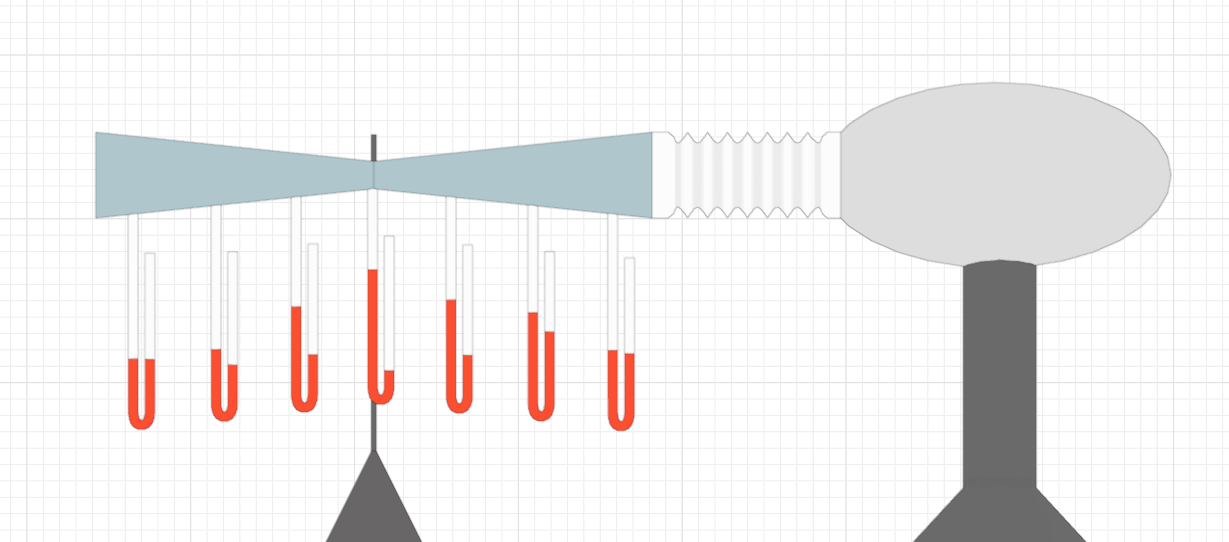
\includegraphics{./Aeromechanik/Protokoll/fig/Venturi_Rohr.png}
    \caption{Drücke am Venturirohr}
    \label{fig:Venturi}
\end{figure}

Dieser Versuch soll die Kontinuitätsgleichung \ref{Kontinuitaetsgleichung} veranschaulichen. Dafür wird ein Gebläse mit einer Venturidüse mit U-Rohr-Manometern verbunden, somit kann man den statischen Druck messen, wobei man damit, zusammen mit der Bernoullischen Gleichung auf die Strömungsgeschwindigkeit schließen kann. Theoretische erwartet man nun den kleinsten statischen Druck in der Einschnürung der Venturidüse, wobei dieser zu den Enden der Düse immer weiter ansteigt. Dadurch kann man darauf schließen, dass die Strömungsgeschwindigkeit in der Mitte der Düse am größten ist, während sie zu den Rändern hin abfällt. Im Experiment lässt sich dieses Verhalten auch deutlich erkennen, allerdings lässt sich auch eine Abweichung von der Theorie an den beiden Enden der Düse erkennen. Was einerseits auf eine Verwirbelung am Auslass der Düse hinweist, aber auch am Einlass der Düse. Dies lässt sich mit dem gebogenen Anschluss zum Gebläse begründen, da man so keine näherungsweise laminare Strömung erzeugen kann, wie sie von der Kontinuitätsgleichung \ref{Kontinuitaetsgleichung} gefordert ist. Trotzdem zeigt das Experiment eindrucksvoll, dass die Kontinuitätsgleichung für laminare Strömungen, wie sie in der Mitte der Düse näherungsweise vorhanden ist, erfüllt ist.

\section{Aerodynamisches Paradoxon}

Die teilweise nicht intuitiven Gesetzmäßigkeiten der Aeromechanik sollen in diesem Versuch gezeigt werden, dafür wird Druckluft axial zwischen zwei eng aneinander liegenden Kreisscheiben ein geströmt. Anders als vielleicht intuitiv erwartet werden die zwei Scheiben nun nicht auseinander gedrückt, sondern aneinander gezogen. Diese Phänomen lässt sich mit Hilfe der Bernoullischer Gleichung \ref{Bernoullische Gleichung} erklären, dadurch, dass die Luft zwischen den Scheiben bewegt ist, sinkt der statische Druck, da der Gesamtdruck konstant ist, ab. Da nun der Umgebungsdruck größer ist, als der Druck zwischen den beiden Kreisscheiben, werden diese nun aneinander gedrückt. Dass der statische Druck bei bewegter Luft im Vergleich zu nicht bewegter oder langsamerer bewegter Luft bei konstantem Gesamtdruck abfällt, findet unter anderem auch bei Tragflächen von Flugzeugen Verwendung.